\chapter{Modelo de Jaynes-Cummings}
\label{ch3_jcm}

%CAMBIAR ESTO PARA PERSONALIZARLO A MI GUSTO
\pagestyle{fancy}
\fancyhf{}
\fancyhead[LE]{\nouppercase{\rightmark\hfill}}
\fancyhead[RO]{\nouppercase{\leftmark\hfill}}
\fancyfoot[LE,RO]{\hfill\thepage\hfill}

En este capitulo analizaremos en profundidad la din\'amica y los aspectos teoricos mas importantes 
del modelo de Jaynes-Cummings, abordando el problema tanto desde un lado te\'orico, como desde
el lado computacional, necesario para resolver la din\'amica en sistemas abiertos.
Primero se trabajar\'a en el modelo de un átomo en una cavidad, se analizar\'an los casos importantes,
y se explicar\' la din\'amica del problema. Esto es importante para comprender conceptualmente como
interact\'uan fundamentalmente la materia y la luz, y nos sirve para conseguir buena intuici\'on del
problema de dos átomos. Tambien se ver\'a la influencia del entorno sobre la cavidad, permitiendo
perdida (o absorci\'on) de fotones, y tambien el bombeo coherente que puede excitar espontaneamente
al átomo. \newline

\section{Modelo y aproximaciónes}
Comencemos entonces por el paradigmatico modelo de 1 átomo. El modelo de Jaynes-Cummings consiste en describir la interacción entre la materia y la luz de manera cuantica, y el experimento mas sencillo consta de un átomo de dos niveles atrapada en una cavidad. La simpleza del modelo surge de las aproximaciónes e hipotesis que se hacen, en primer lugar, el campo electromagnetico dentro de la cavidad puede en principio tener infinitos modos, pero para simplificar se considera solo un modo. 
Entonces tenemos un Hamiltoniano ($\hbar = 1$)

\begin{align*}
\hat H & = \hat H_A + \hat H_C + \hat H_{int}  \\
\hat H_A &= \omega \frac{\sigma_z}{2} \\
\hat H_C &= \epsilon \hat a^\dagger\hat a = \epsilon \hat n \\
\hat H_{int} &= -i g (\hat\sigma_-+\hat \sigma_+)(\hat a - \hat a^\dagger)
\end{align*}

donde $\epsilon$ y $\omega$ son las freccuencias naturales de la cavidad y del átomo respctivamente. Los operadores $\hat a$ y $\hat a^\dagger$ son los operadores de aniquilaci\'on y creaci\'on fot\'onicos de la cavidad y $\hat n =a^\dagger a$ es el operador de n\'umero de la cavidad, y $\hat \sigma_z$ es el operador de pauli. Los estados del átomo de dos niveles los llamamos $\ket{g}$ y $\ket{e}$ al estado ground y excitado respectivamente, y con esta notación los operadores $\sigma_\pm = (\sigma_x\pm i\sigma_y)/2$ son los operadores de subida y bajada atomicos. 
La interacci\'on es complicada, y para simplificar lo que se hace es usar la representaci\'on de interacci\'on, y uno encuentra que hay dos frecuencias, una que llamamos \textit{rotante} y es la diferencia entre las frecuencias caracteristicas $\epsilon-\omega$, y la otra frecuencia es la suma $\epsilon+\omega$. La aproximación de onda rotante vale cuando las frecuencias son similares $\epsilon\sim\omega$, y consta de despreciar la dinamica de los terminos contrarrotantes, ya que oscilan muy rapidamente en comparación con los terminos rotantes, y entonces podemos promediar los efectos de los terminos rapidos. Entonces al aplicar esta aproximación, justificada cuando $\epsilon\sim\omega$ y $g \ll \epsilon,\omega$ se obtiene el hamiltoniano de JC \ref{}\textcolor{red}{ludmi 49}
\begin{equation}
    H_{JC}=\epsilon a^\dagger a + \omega \sigma_z/2 + g(a^\dagger\sigma_-+a\sigma_+)
\end{equation} 
La interpretaci\'on de la interacci\'on en este caso es clara, las dos opciones son que el átomo suba un nivel de energ\'ia y en consecuencia la cavidad pierda un fot\'on, o que el átomo baje un nivel, y la cavidad gane una excitaci\'on. Este Hamiltoniano conserva el n\'umero total de excitaciones $\hat N= \hat n + \hat \sigma$. En este momento es usual aplicar una transformación unitaria $K=\exp{-i\omega t(a ^\dagger a + \sigma_z/2)}$ sobre el Hamiltoniano que queda 
\begin{equation}\label{eq3:hamiltoniano jcm}
    H=\frac{\Delta}{2}\sigma_z+g(a^\dagger \sigma_-+a \sigma_+)
\end{equation}
donde $\Delta = \epsilon - \omega$ es el \textit{detunning} entre las frecuencias de la cavidad y el átomo. Un ejemplo de esto es un átomo de Rydberg metido en una cavidad \ref{}, o ... \textcolor{red}{BUSCAR EJEMPLOS}.
Como el Hamiltoniano conserva la cantidad de excitaciones es oportuno agrupar los estados en funci\'on de la cantidad de excitaciones: $\{\ket{g,n},\ket{e,n-1}\}$. En esta base el Hamiltoniano se diagonaliza por bloques, ya que las interacciones conservan la cantidad total de excitaciones, entonces los elementos de matriz entre estados con diferente cantidad de excitaciones se corresponde
\begin{align*}
    [H,\hat N]=0 \implies & \bra{N'}H \hat N \ket{N} = \bra{N'}\hat N H \ket{N} \\
    & N \bra{N'}H  \ket{N} = N' \bra{N'}H \ket{N} \\
    & \implies \bra{N'}H \ket{N} = \begin{cases}
        0 \text{ , si } N' \neq N \\
        \bra{N}H \ket{N} \text{ , si } N'=N
    \end{cases}
\end{align*}
donde $\ket{N}$ es un estado con $N$ excitaciones totales. Entonces para resolver el problema solo tenemos que mirar el subespacio de 2x2 de n excitaciones, cuyo Hamiltoniano es
\begin{equation}
    H_n=\begin{pmatrix}
        -\frac{\Delta}{2} & g \sqrt{n} \\
        g \sqrt{n} & \frac{\Delta}{2} 
    \end{pmatrix}
\end{equation}
Resolvemos el problema de autovalores y autovectores y obtenemos
\begin{equation}
    \begin{aligned}
        \ket{\psi^n_-} & = \cos \frac{\theta_n}{2}\ket{g,n}-\sin \frac{\theta_n}{2}\ket{e,n-1} \\
        \ket{\psi^n_+} & = \sin \frac{\theta_n}{2}\ket{g,n}+\cos \frac{\theta_n}{2}\ket{e,n-1}        
    \end{aligned}
\end{equation}
con $E_{\pm}^n=\pm \frac{\Omega}{2}$ las autoenergias y $\Omega_n=\sqrt{\Delta^2+4g^2n}$ la frecuencia de Rabi del sistema, $\cos \theta_n=\frac{\Delta}{\Omega_n}$ modulando la superposici\'on de estados. 
\begin{figure}
    \centering
    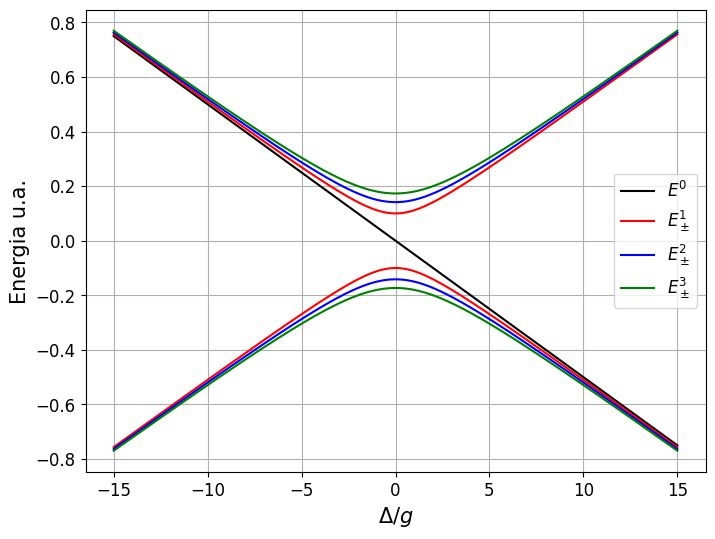
\includegraphics[width=0.7\textwidth]{figuras/ch3/relacion energia detunning jcm simple.png}
    \caption{Relaci\'on energ\'ia detunning para el modelo de Jaynes-Cummings. La diferencia de energ\'ia entre los estados de un mismo nivel para $\Delta=0$ es $2g\sqrt{n}$.}
    \label{fig:relación energia detunning jcm1}
\end{figure}
En la figura \ref{fig:relación energia detunning jcm1} se observan las curvas de energ\'ia en funci\'on del detunning para diferentes niveles. Lo primero que tenemos que observar es que en el caso resonante, es decir $\Delta=0$, los autoestados del sistema son los estados maximamente entrelazados de Bell
\begin{equation}
    \ket{\psi_\pm^n}=\frac{1}{\sqrt{2}}(\ket{gn}\pm\ket{e,n-1})
\end{equation} 
y la diferencia de energ\'ia entre los autoestados es $\Delta E^n =E^n_+-E^n_-=2g\sqrt{n}$. En el caso muy lejos de resonancia podemos asumir que $\Delta \gg g $, y entonces los autoestados coinciden en este l\'imite con los estados de la base, 
\begin{equation}
    \begin{aligned}
        \ket{\psi^n_+}=\ket{e,n-1} \\
        \ket{\psi^n_-}=\ket{g,n}
    \end{aligned}
\end{equation}
Ac\'a hay una sutileza, y es que si $\Delta>0$, entonces $\ket{e,n-1}$ es el estado de mayor energ\'ia y la notaci\'on coincide con la energ\'ia, pero si $\Delta<0$ entonces el estado $\ket{\psi^n_+}$ es el estado de menor energ\'ia. 
Un efecto interesante es que en el caso de alta desinton\'ia, podemos calcular la diferencia entre la energía del autoestado exacto del Hamiltoniano $\ket{\psi_\pm^n}$ y la energía asintotica a la que tiende, que es la energía de los estados de la base $\ket{g,n},\ket{e,n-1}$. Esta diferencia ... \textcolor{red}{VOLVER A ESTO Y VER SI DEJARLO O SACARLO. EVENTUALMENTE COMPLETAR.}
\begin{equation}
    \begin{aligned}
        \Delta E_{e,n-1}=E_+^n-E^{(0)}_{e,n-1}=\frac{g^2}{\Delta}n
        \Delta E_{g,n}=E_-^n-E^{(0)}_{g,n}=-\frac{g^2}{\Delta}n
    \end{aligned}
\end{equation}
El resultado importante de esta diferencia de energias es que aun en ausencia de fotones en la cavidad $n=0$, hay una diferencia entre las energias entre el Hamiltoniano del átomo, y del $H_{JC}$. Este efecto es el \textit{Lamb Shift} y nos dice que el vac\'io electromagnetico induce un corrimiento en la energ\'ia de los estados. Esto es importante notarlo, porque para el caso de dos átomos tambien est\'a manifiesto.

\subsection{Fase geométrica en el JCM}
Vamos a analizar la fase de Berry y la fase geométrica en la aproximación cinemática.
\subsubsection{Fase de Berry}
Para ver la fase de berry tenemos que tener un parámetro de control en el Hamiltoniano, el cual varía lentamente. Para esto necesitamos aplicar una transformación unitaria de corrimiento de fase al Hamiltoniano original \ref{eq3:hamiltoniano jcm} $R=\exp{-i\Omega a^\dagger a}$, que queda
\begin{equation}
    H=\frac{\Delta}{2}\sigma_z+g(a^\dagger \sigma_e^{-i\Omega}-+a\sigma_+e^{i\Omega})
\end{equation}
que ahora depende explicitamente del parámetro externo de control $\Omega$. Los autoestados de este nuevo Hamiltoniano se obtienen aplicando esta misma transformación sobre los autoestados del Hamiltoniano original. Si el parámetro de control varia lentamente entre 0 y $2\pi$, entonces estamos dentro de las hipotesis propuestas por Berry, y podemos calcular la fase de Berry mediante la ecuación \ref{eq2:fg berry}:
\begin{equation}
    \psi_a^n=i\oint_Cd\Omega\bra{\psi_\pm^n}R(\Omega)^\dagger \frac{d}{d\Omega}\ket{\psi_\pm^n}=\pi(1\pm \cos(\theta_n))
\end{equation}

que es no trivial incluso para $n=0$, lo que nos dice que incluso el vacio electromagnetico introduce una corrección en la fase de Berry.
\subsubsection{Aproximación Cinemática}
Para comparar ambos metodos, ahora vamos a calcular la fase geométrica utilizando la aproximación cinemática aunque este abordaje es más general de lo necesario en este caso.
Si se considera que el estado inicial es un atuoestado del Hamiltoniano, como los estados $\ket{\psi_\pm^n}$, entonces la fase geométrica en este caso se anula. Pero si se considera un estado inicial, por ejemplo $\ket{\psi(0)}=\ket{e,n}$, entonces el estado a tiempo $t$ resulta
\begin{equation}\label{eq3:fg berry jcm}
    \ket{\psi(t)}=(\cos^2\theta_ne^{-iE_+^nt}+\sin^2\theta_ne^{iE_+^nt})\ket{e,n}-i \sin\theta_n\sin(E_+^nt)\ket{g,n+1}
\end{equation}
La fase geometrica acumulada \ref{eq2:fg cinematica unitaria} es
\begin{equation}\label{eq3:fg unitaria jcm}
    \phi_u[C]=-\pi(1-\cos\theta_n)\frac{t}{T} +\arg\left\{ 1+e^{2\pi i \frac{t}{T}}\frac{\Omega_n-\Delta}{\Omega_n+\Delta} \right\}
\end{equation}
con $T=\frac{2\pi}{\Omega_n}$ es un período correspondiente a la frecuencia de Rabi $\Omega_n$. Esta expresión y la antrior \ref{eq3:fg berry jcm}, deberian coincidir cuando $t=T$, que se corresponde con un ciclo cerrado. En este caso ($t=T$) se obtiene
\begin{equation}
    \phi_u=-\pi(1-\cos\theta_n)
\end{equation}
La diferencia de signos se puede explicar comparando las curvas descritas por la esfera de Bloch para cada evolución. 
\begin{figure}[H]
    \centering
    \begin{subfigure}[h]{0.49\textwidth}
        \centering
        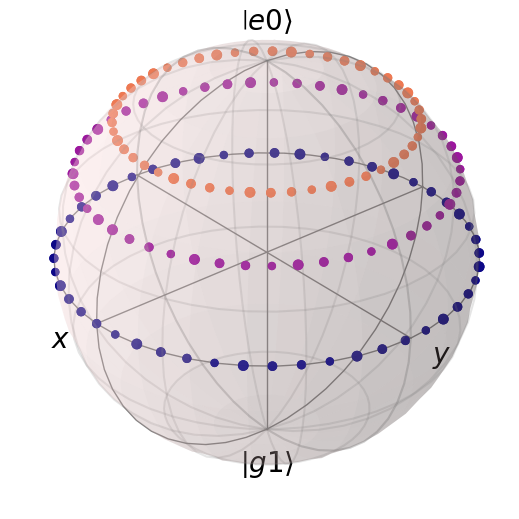
\includegraphics[width=\textwidth]{figuras/ch3/bloch berry.png}
        \caption{Evolución adiabática} 
        \label{fig3:bloch berry}
    \end{subfigure}
    \hfill
    \begin{subfigure}[h]{0.49\textwidth}
        \centering
        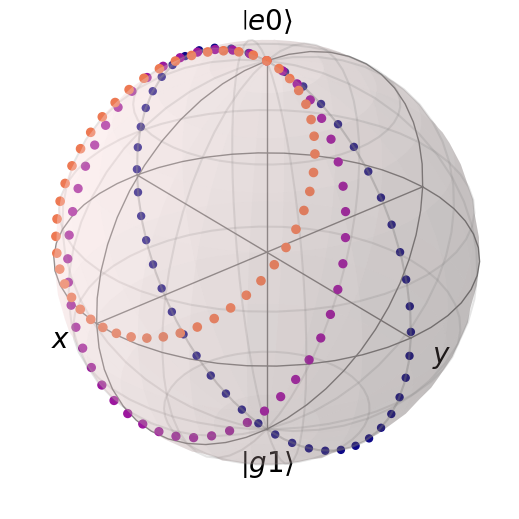
\includegraphics[width=\textwidth]{figuras/ch3/bloch cinematica.png}
        \caption{Enfoque cinemático}
        \label{fig3:bloch cinematica}
    \end{subfigure}
    \caption{}
    \label{fig3:esfera de bloch jcm}
\end{figure}
En el caso \ref{eq3:fg berry jcm}, correspondiente a la figura \ref{fig3:bloch berry}, los autoestados son los autoestados $R(\Omega)\ket{\psi_\pm^n}=e^{-i\Omega \hat n}\ket{\psi_\pm^n}$, entonces al variar $\Omega\in [0,2\pi]$ la trayectoria es simplemente un circulo en la esfera de Bloch. En cambio, en el segundo caso, si preparamos el sistema inicialmente en el estado $\ket{e,n}$ y lo dejamos evolucionar por la acción de H durante un tiempo, la trayectoria ahora no son circulos horizontales en la esfera, sino que parten del polo norte, que es el estado $\ket{e,n}$, y luego hace una trayectoria ovalada, para finalmente volver al punto inicial de partida a un tiempo $t=T$. La diferencia en el signo se explica a travez de la transformación que nos lleva de una curva a la otra. Para esto, necesitamos de una rotacion rigida, y una inversion de la parametrizacion, por su parte, esta ultima, introduce un signo negativo, cosa que se ve claramente en la ecuacion \ref{eq3:fg unitaria jcm} al cambiar $t\rightarrow -t$.

\textcolor{red}{aca puedo intentar de agregar el caso con medio kerr. Creo que no es tan complicado y el problema de autocosas ya lo tengo medio resuelto en papel desde hace un tiempo, pero lo tengo que revisar a ver si esta bien y lo tengo que completar, pero puede estar bueno para entender que le hace a la FG desde el vamos.}

\section{JCM disipativo}


Habiendo desarrollado el análisis de la fase geométrica acumulada por el sistema átomo-cavidad en la situación ideal de completo aislamiento, se aborda ahora el estudio para el escenario más realista en el que el mismo sistema se encuentra en interacción con un entorno. El problema se trata para la implementación específica en estructuras semiconductoras, en las que un punto cuántico (al cual se sigue, sin embargo, refiriendo como átomo o sistema de dos niveles) se ubica en una nano o micro-cavidad.

Siguiendo \cite{80}, en este capítulo se estudia en detalle la fase geométrica acumulada en un modelo de Jaynes-Cummings disipativo, como caso paradigmático dentro del campo de la electrodinámica en cavidades. Se considera que los principales mecanismos por los cuales el sistema “átomo + modo” interactúa con el entorno son el flujo de fotones a través de las paredes de la cavidad y el continuo e incoherente bombeo del sistema de dos niveles, lo que conforma un escenario frecuente en electrodinámica de cavidades semiconductoras \cite{81,82,83}. 

Para poder modelar estos mecanismos, se emplea la ecuación maestra fenomenológica de Lindblad
\begin{equation}\label{eq3:lindblad}
\dot{\rho}(t) = -i [H, \rho(t)] + \frac{1}{2} \sum_\alpha \big( 2L_\alpha \rho(t) L_\alpha^{\dagger} - \{ L_\alpha^{\dagger}L_\alpha, \rho(t) \} \big),
\end{equation}

, despreciando otros procesos con menor influencia en la dinámica como el desfasaje puro o el bombeo de fotones del entorno en la cavidad, considerando además que el entorno se halla a temperatura cero. Los operadores de Lindblad

\begin{equation}
L_\gamma = \sqrt{\gamma} \ a
\end{equation}
\begin{equation}
L_p = \sqrt{p} \ \sigma_+
\end{equation}

,representan la pérdida de fotones y el bombeo continuo e incoherente del átomo, respectivamente, con los parámetros $\gamma$ y $p$ denominados tasa de pérdida de fotones y amplitud del bombeo. 

El bombeo sobre el átomo es siempre secundario frente a la pérdida de fotones, lo cual nos da las relaciones $\frac{p}{g},\frac{p}{\gamma} \ll 1$, y la relación entre $\gamma$ y $g$ da lugar a dos regimenes que se diferencian con claridad \cite{50}-\cite{54}. El regimen de acoplamiento fuerte (SC o Strong Coupling) es cuando la interacción átomo-cavidad es mas fuerte que la disipación del entorno, es decir $\gamma /g <1$. En el caso contrario $\gamma/g>1$ estamos en el régimen de acoplamiento débil (WC o Weak Coupling). Para no generar confusiones, hay que destacar que en general, cuando en la literatura se habla de acoplamientos fuertes y debiles, se refiere a la interacción entre las partes del mismo sistema, pero en este caso, se esta haciendo referencia a la interacción del sistema con el entorno EN COMPARACIÓN con la interacción interna del sistema.

En esta ocación nos interesa resolver el problema restringiendonos al subespacio donde el átomo puede estar en cualquiera de sus dos estados, y nos restringimos al caso en donde la cavidad tiene 1 o 2 fotones, en consecuencia, se restringe el estudio a un subespacio truncado cuya base son los estados $\{ \ket{0}=\ket{g,0} ; \ket{1}=\ket{e,0} ; \ket{2}=\ket{-,1} \}$. Desarrollando explicitamente el sistema de ecuaciones dadas por la ecuación de Lindblad \ref{eq3:lindblad}, obtenemos que los elementos $\rho_{0i}$ quedan desacoplados de los demas:

\begin{equation}
    \begin{aligned}
        \dot \rho_{01} & =-\frac{p}{2} \rho_{01}+i\Delta\rho_{01}+ig\rho_{02} \\
        \dot \rho_{02} & =-\frac{p}{2} \rho_{02}-\gamma \rho_{02}+ig\rho_{01}
    \end{aligned}
\end{equation}
,con lo cual, si inicialmente los elementos de matriz $\rho_{0i}(0)=0$, permanecerán así durante toda la evolución del sistema. Para hacer una analogía y realizar una comparación con el caso unitario, se estudia la condición inicial $\rho(0)=\ketbra{e,0}{e,0}$, que satisface esta condición, de manera que se espera que el estado $\rho(t)$ exciba una estructura diagonal por bloques. El primer bloque de 1x1 representando al estado $\ket{0}$, y luego un bloque de 2x2 que describe la dinámica entre los estados $\ket{1}$ y $\ket{2}$. Las ecuaciones son
\begin{equation}
\begin{aligned}
\dot{\rho}_{00} &= -p \rho_{00} + \gamma \rho_{22}, \\
\dot{\rho}_{11} &= -i g (\rho_{21} - \rho_{12}) + p \rho_{00}, \\
\dot{\rho}_{22} &= -i g (\rho_{12} - \rho_{21}) - \gamma \rho_{22}, \\
\dot{\rho}_{12} &= -i g (\rho_{22} - \rho_{11}) - i \Delta \rho_{12} - \frac{\gamma}{2} \rho_{12}.
\end{aligned}
\end{equation}

que se resuelven numericamente para acceder al estado $\rho(t)$ a tiempo $t>0$. 

\textbf{[Placeholder para Figura: Evolución dinámica de elementos de matriz]}

El análisis de esta sección permite establecer la relación entre los efectos de disipación y la acumulación de la fase geométrica, así como determinar las condiciones bajo las cuales el sistema mantiene coherencia cuántica suficiente para aplicaciones experimentales.
